\RequirePackage{amsmath}
\RequirePackage{fix-cm}
\documentclass{svmono}

\def\ColoredLinks{}
%%%%%%%%%%%%%%%%%%%%%%%%%%%%%%%%%%%%%%%%%%%
% Alexanders Standardmacros - Version 3.0 %
%%%%%%%%%%%%%%%%%%%%%%%%%%%%%%%%%%%%%%%%%%%





%%%%%%%%%%%%%%%%%%%%%%%%%%%%%%%%%%%%%%%%%%%%%%%%
%  Farben für Links definieren                 %
%%%%%%%%%%%%%%%%%%%%%%%%%%%%%%%%%%%%%%%%%%%%%%%%

\ifdefined\ColoredLinks
  \def\linkColorLinkR{0}
  \def\linkColorLinkG{0}
  \def\linkColorLinkB{0.55}
	\def\linkColorCiteR{0}
  \def\linkColorCiteG{0}
  \def\linkColorCiteB{0.55}
	\def\linkColorUrlR{0}
  \def\linkColorUrlG{0}
  \def\linkColorUrlB{0.55}
\else
  \def\linkColorLinkR{0}
  \def\linkColorLinkG{0}
  \def\linkColorLinkB{0}
	\def\linkColorCiteR{0.3}
  \def\linkColorCiteG{0.3}
  \def\linkColorCiteB{0.3}
	\def\linkColorUrlR{0}
  \def\linkColorUrlG{0}
  \def\linkColorUrlB{0}
\fi





%%%%%%%%%%%%%%%%%%%%%%%%%%%%%%%%%%%%%%%%%%%%%%%%
%  Packages einbinden                          %
%%%%%%%%%%%%%%%%%%%%%%%%%%%%%%%%%%%%%%%%%%%%%%%%

%\usepackage{makeidx} - unterschägt manchmal Einträge
\usepackage{imakeidx} % Speziellen Features eigentlicht nicht verwendet, aber hat die makeidx-Fehler nicht
\usepackage[utf8]{inputenc}
\usepackage{amssymb}
\usepackage[ngerman]{babel}
\usepackage{epsf}
\usepackage[dvips]{rotating}
\usepackage{amsmath,amsfonts}
\usepackage[amsmath,thmmarks,noconfig]{ntheorem}
\usepackage{nameref}
\usepackage{hycolor}
\usepackage{hyperxmp}
\usepackage{hyperref}
\hypersetup{pdfauthor={Alexander Herzog},
            pdftitle={Warteschlangensimulator - Kurzeinführung},
            %pdfsubject={},
            %pdfkeywords={},
            pdfproducer={LaTeX},
            pdfcreator={pdfLaTeX},
						pdfcopyright={Copyright Alexander Herzog},
						pdfcontactcity={Clausthal-Zellerfeld},
						pdfcontactpostcode={38678},
						pdfcontactcountry={Deutschland},
						pdfcontactemail={alexander.herzog@tu-clausthal.de},
						pdfcontacturl={https://www.simzentrum.de,https://www.tu-clausthal.de},
						pdflang={de},
						bookmarksnumbered,
						colorlinks=true,
						filecolor=[rgb]{0,0,0},  % \href-Links nicht hervorheben
						linkcolor=[rgb]{\linkColorLinkR,\linkColorLinkG,\linkColorLinkB},
						citecolor=[rgb]{\linkColorCiteR,\linkColorCiteG,\linkColorCiteB},
						urlcolor=[rgb]{\linkColorUrlR,\linkColorUrlG,\linkColorUrlB} %\url{}, nur für E-Mail-Link genutzt
					}
\expandafter\def\expandafter\UrlBreaks\expandafter{\UrlBreaks
  \do\a\do\b\do\c\do\d\do\e\do\f\do\g\do\h\do\i\do\j
  \do\k\do\l\do\m\do\n\do\o\do\p\do\q\do\r\do\s\do\t
  \do\u\do\v\do\w\do\x\do\y\do\z\do\A\do\B\do\C\do\D
  \do\E\do\F\do\G\do\H\do\I\do\J\do\K\do\L\do\M\do\N
  \do\O\do\P\do\Q\do\R\do\S\do\T\do\U\do\V\do\W\do\X
  \do\Y\do\Z}
\usepackage{float}
\usepackage{fancyvrb}
\restylefloat{figure}
\restylefloat{table}
\usepackage{sectsty}
%\allsectionsfont{\fontfamily{cmss}\selectfont} - das führt zu Type 3 Fonts
\allsectionsfont{\sffamily\selectfont}
\usepackage{framed}
\usepackage[toc,page]{appendix}
\renewcommand\appendixname{Anhang}
\let\appendixtocname\appendixname\let\appendixpagename\appendixname
\usepackage[T1]{fontenc} % aus der pdf kopierbare Umlaute
\usepackage{eurosym}
\usepackage{longtable}

\usepackage{graphicx}
\usepackage[export]{adjustbox}




%%%%%%%%%%%%%%%%%%%%%%%%%%%%%%%%%%%%%%%%%%%%%%%%
%  Rotierte Tabellenüberschriften              %
%%%%%%%%%%%%%%%%%%%%%%%%%%%%%%%%%%%%%%%%%%%%%%%%

\usepackage{adjustbox}
\usepackage{array}
\usepackage{booktabs}
\usepackage{multirow}

\newcolumntype{R}[2]{%
    >{\adjustbox{angle=#1,lap=\width-(#2)}\bgroup}%
    l%
    <{\egroup}%
}
\newcommand*\rot{\multicolumn{1}{|R{90}{1em}|}}





%%%%%%%%%%%%%%%%%%%%%%%%%%%%%%%%%%%%%%%%%%%%%%%%
%  Symbole definieren                          %
%%%%%%%%%%%%%%%%%%%%%%%%%%%%%%%%%%%%%%%%%%%%%%%%

\newcommand{\setH}{\mathbb{H}}
\newcommand{\setC}{\mathbb{C}}
\newcommand{\setR}{\mathbb{R}}
\newcommand{\setQ}{\mathbb{Q}}
\newcommand{\setZ}{\mathbb{Z}}
\newcommand{\setN}{\mathbb{N}}
\newcommand{\comp}{\complement}
\newcommand{\Umg}{{\cal U}}

\newcommand{\calA}{{\cal A}}
\newcommand{\calB}{{\cal B}}
\newcommand{\calC}{{\cal C}}
\newcommand{\calD}{{\cal D}}
\newcommand{\calE}{{\cal E}}
\newcommand{\calF}{{\cal F}}
\newcommand{\calG}{{\cal G}}
\newcommand{\calH}{{\cal H}}
\newcommand{\calI}{{\cal I}}
\newcommand{\calJ}{{\cal J}}
\newcommand{\calK}{{\cal K}}
\newcommand{\calL}{{\cal L}}
\newcommand{\calM}{{\cal M}}
\newcommand{\calN}{{\cal N}}
\newcommand{\calO}{{\cal O}}
\newcommand{\calP}{{\cal P}}
\newcommand{\calQ}{{\cal Q}}
\newcommand{\calR}{{\cal R}}
\newcommand{\calS}{{\cal S}}
\newcommand{\calT}{{\cal T}}
\newcommand{\calU}{{\cal U}}
\newcommand{\calV}{{\cal V}}
\newcommand{\calW}{{\cal W}}
\newcommand{\calX}{{\cal X}}
\newcommand{\calY}{{\cal Y}}
\newcommand{\calZ}{{\cal Z}}

\def\arccot{\mathop{\rm arccot}}
\def\Arcoth{\mathop{\rm Arcoth}}
\def\Arsinh{\mathop{\rm Arsinh}}
\def\Artanh{\mathop{\rm Artanh}}
\def\Arcosh{\mathop{\rm Arcosh}}

\def\d{{\rm d}}
\def\dx{\d x}
\def\dy{\d y}
\def\dz{\d z}
\def\dt{\d t}
\def\euler{\mathrm{e}}

\def\id{{\rm id}}
\def\Kern{{\rm Kern}}

\def\ra{\Rightarrow}

\def\oversym#1#2{\mathop{#1}\limits^{#2}}
\def\Inneres#1{\oversym{#1}\circ}


\def\TO#1{\oversym\longrightarrow{#1}}
\def\RA#1{\oversym\Longrightarrow{#1}}
\def\IFF#1{\oversym\iff{#1}}
\def\gleich#1{\oversym={#1}}

\def\oBdA{o.\,B.\,d.\,A.\ }

\renewcommand{\qed}{\begin{flushright} $\square$ \end{flushright}}

\def\Definition#1{{\bf #1}}

\def\E{{\bf E}}
\def\Var{{\bf Var}}
\def\Std{{\bf Std}}
\def\CV{{\bf CV}}
\def\SCV{{\bf SCV}}





%%%%%%%%%%%%%%%%%%%%%%%%%%%%%%%%%%%%%%%%%%%%%%%%
%  Umgebungen definieren                       %
%%%%%%%%%%%%%%%%%%%%%%%%%%%%%%%%%%%%%%%%%%%%%%%%

%\theoremstyle{changebreak}
%\theoremheaderfont{\normalfont\bfseries}
%\theoremseparator{:}
%\theoremsymbol{}
%\newtheorem{definition}{Definition}[chapter]
%\newtheorem{satz}[definition]{Satz}
%\newtheorem{hilfssatz}[definition]{Hilfssatz}
%\newtheorem{lemma}[definition]{Lemma}
%\newtheorem{beispiel}[definition]{Beispiel}
%\newtheorem{beispiele}[definition]{Beispiele}
%\newtheorem{bezeichnung}[definition]{Bezeichnung}
%\theorembodyfont{\rmfamily}
%\newtheorem{bemerkung}[definition]{Bemerkung}
%\newtheorem{vereinbarung}[definition]{Vereinbarung}
%\newtheorem{folgerung}[definition]{Folgerung}
%\theoremheaderfont{\normalfont\bfseries}
%\theoremstyle{nonumberchangebreak}
%\theorembodyfont{\rmfamily}
%\theoremsymbol{$\blacksquare$}
%\newtheorem{beweis}{Beweis}
%\theoremsymbol{}





%%%%%%%%%%%%%%%%%%%%%%%%%%%%%%%%%%%%%%%%%%%%%%%%
%  Standard epsilon durch schöneres ersetzen   %
%%%%%%%%%%%%%%%%%%%%%%%%%%%%%%%%%%%%%%%%%%%%%%%%

\def\epsilon{\varepsilon}





%%%%%%%%%%%%%%%%%%%%%%%%%%%%%%%%%%%%%%%%%%%%%%%%
%  Verbatim-Umgebungen für verschiedene Zwecke %
%%%%%%%%%%%%%%%%%%%%%%%%%%%%%%%%%%%%%%%%%%%%%%%%

\DefineVerbatimEnvironment{ExcelVerbatim}{Verbatim}{frame=single,label=Excel-Befehl,fontsize=\small}
\DefineVerbatimEnvironment{ExcelVerbatimWithMath}{Verbatim}{frame=single,label=Excel-Befehl,commandchars=\\\{\},codes={\catcode`$=3\catcode`^=7},fontsize=\small}
\DefineVerbatimEnvironment{ExcelVerbatimWithFormat}{Verbatim}{frame=single,label=Excel-Befehl,fontsize=\small,commandchars=\\\{\}}
\DefineVerbatimEnvironment{RVerbatim}{Verbatim}{frame=single,label=R-Code,fontsize=\small}
\DefineVerbatimEnvironment{ExcelMacroVerbatim}{Verbatim}{frame=single,label=Excel-Makro,fontsize=\small} % ,numbers=left
\DefineVerbatimEnvironment{ExcelMarcroVerbatimWithMath}{Verbatim}{frame=single,label=Excel-Makro,commandchars=\\\{\},codes={\catcode`$=3\catcode`^=7},fontsize=\small}
\DefineVerbatimEnvironment{ExcelMacroVerbatimWithFormat}{Verbatim}{frame=single,label=Excel-Makro,fontsize=\small,commandchars=\\\{\}}
\newcommand{\sub}[2]{{#1_#2}}

\newcommand{\newlinesymbol}{\rotatebox[origin=c]{270}{$\curvearrowright$}}





%%%%%%%%%%%%%%%%%%%%%%%%%%%%%%%%%%%%%%%%%%%%%%%%
%  Formatierungen                              %
%%%%%%%%%%%%%%%%%%%%%%%%%%%%%%%%%%%%%%%%%%%%%%%%

%\def\emphasis#1{\textbf{#1}}
%\def\emphasisBFOnly#1{\textbf{#1}}
\def\emphasis#1{\emph{#1}}
\def\emphasisBFOnly#1{#1}

\def\emphasisIT#1{\textit{#1}}
\def\emphasisEnglish#1{\textit{#1}}

%\font\deutschfont=suet14
%\def\deutsch#1{\hbox{\deutschfont #1}}

\parindent0pt
\parskip5pt

%\oddsidemargin4.6mm
%\evensidemargin-5.4mm
%\textwidth160mm
\usepackage{xcolor}
\usepackage{lmodern}
\usepackage{wrapfig}
\usepackage[english]{keystroke}
\textwidth160mm
\textheight220mm
\oddsidemargin0mm
\evensidemargin0mm
\topmargin0mm

\def\cmd#1{\textbf{"\texttt{#1}"}}
\def\cm#1{\textbf{\texttt{#1}}}

\begin{document}

\hypersetup{pageanchor=false}
\thispagestyle{empty}
\vskip5cm {\Huge\textbf{Lecturer's guide}}
\vskip.5cm \hrule
\vskip.5cm {\large \textsc{Alexander Herzog} (\href{mailto:alexander.herzog@tu-clausthal.de}{alexander.herzog@tu-clausthal.de})}
\IfFileExists{../../Warteschlangennetz-mittel.png}{
\vskip2cm \centerline{\fbox{\includegraphics[width=16cm]{../../Warteschlangennetz-mittel.jpg}}}
}{}
\vskip2cm {\color{gray}
This reference refers to version 4.6.0
 of Warteschlangensimulator.\\
Download address: \href{https://a-herzog.github.io/Warteschlangensimulator/}{https://a-herzog.github.io/Warteschlangensimulator/}.
}

\vfill
\pagebreak

\setcounter{page}{1}

This document summarizes a number of information for lecturers who want to use Warteschlangensimulator in teaching. It describes which competences of the students are required for the use of the simulator, which notation is used in the simulator and which questions are particularly suitable as introductory examples.



\chapter{Prerequisites}

\section{Prerequisites for using Warteschlangensimulator}

Warteschlangensimulator is aimed for the three fields of application: industrial use, research and teaching. For the use in companies, e.\,g.\ database connections as well as the integration into reporting systems are important. For the investigation of complex research questions, a high simulation speed and the possibility to run the simulator without graphical output on a remote (Linux) compute server are of particular importance. For use in teaching, the simulator has a program interface that can be used as intuitively as possible, as well as numerous help and explanation texts.

With the help of Warteschlangensimulator, questions from queueing theory, for which no exact formulas may be known, can be investigated. Although an attempt is made to keep the complex mathematical relations and also the informatic concepts of the event-oriented, stochastic simulation in the background as much as possible, some basic knowledge is still necessary for the successful use of the simulator:

\paragraph{Stochastics}~\\
Knowledge of the basic concepts of probability is necessary for building models and for interpreting the results. Specifically, the following terms should be known:

\begin{itemize}
\item
Concept of probability (e.\,g., for the branching of customer flows in different directions according to different probabilities); related to this, the concept of rate (as unnormalized probability).
\item
Essential discrete and continuous probability distributions; in this context, the meaning of density and distribution function.
\item
Expected values, standard deviations, coefficient of variation
\end{itemize}

The conversion between expected value and standard deviation on the one hand and the respective distribution parameters on the other hand is done automatically in the simulator whenever possible, i.\,e.\ the exact knowledge of the formulas for calculating the distribution parameters from the characteristics (and vice versa) is not necessary for most commonly used distributions. However, a general understanding of what e.\,g.\ expected value and standard deviation actually mean in relation to a probability distribution is very much necessary.

\paragraph{Queueing theory}~\\
Less concrete formulas are needed from the queueing theory, but much more the essential terminology. Specifically, the following terms are important for the use of the simulator:

\begin{itemize}
\item
General structure of a queueing model (arrival process, waiting room, service desk; objects: customers, operators)
\item
Characterization of the arrival process (arrival rate and inter-arrival times)
\item
Exponential distribution (including its property of memorylessness and explanation of why this is often appropriate for arrival processes).
\item
Characterization of the service process (number of operators, service rate and service time)
\item
Typical probability distributions for the service times (e.\,g.\ log-normal distribution)
\item
Common characteristics (workload, utilization, waiting time, residence time, number of customers in the queue or in the system)
\end{itemize}

The \textsc{Markov} theory and also the \textsc{Kendall} notation are not needed for the use of the simulator and also for the interpretation of the results. Of course, it can be didactically interesting to explain e.\,g.\ the \textsc{Erlang} formulas in the introduction to the simulation methods and to introduce the \textsc{Markov} theory for this purpose and the \textsc{Kendall} notation for the classification of simple models.

\paragraph{Beyond queueing theory}~\\
In classical queueing theory, mainly models that can be described in the \textsc{Kendall} notation are discussed. For an analytical consideration, the complete coverage of the possibilities of the \textsc{Kendall} notation already represents a very large challenge\footnote{siehe z.\,B.\ Shortle, John F., et al. \emph{Fundamentals of queueing theory}. Vol.\ 399. John Wiley \& Sons, 2018.}. However, the capabilities of simulation models go far beyond these models.

Therefore, in order to identify interesting questions for the later use of the simulator, it is useful to explain in advance some properties relevant in real queueing systems:

\begin{itemize}
\item
Impatience of customers
\item
Examining different customer types with e.\,g.\ different priorities or a routing to different sub-models (because e.\,g.\ not all call center agents can serve all customer types)
\item
Set-up times when changing from one customer type to another on one machine
\item
Loops either due to rework or due to redialing in call centers
\end{itemize}

\paragraph{Event oriented simulation}~\\
Warteschlangensimulator is a classical event-oriented, stochastic simulator. The basis for the fast processing of the events that successively arise during the simulation is an efficient event management. These architectural considerations are not visible to the user, and knowledge of these concepts is not required for meaningful use of the simulator.

Nevertheless, in a more informatic view, of course, one can also take a look at these concepts\footnote{siehe auch \href{https://github.com/A-Herzog/Warteschlangensimulator/wiki/Architecture}{github.com/A-Herzog/Warteschlangensimulator/wiki/Architecture}}:
\begin{itemize}
\item
Which operations occur how often? (Insertion of events with arbitrary execution times and removal of the event with the smallest execution time each very often; removal of events (not to be processed) with arbitrary execution times rarely).
\item
How can the smallest possible $O$ classes be achieved for the operations? (For the processing of the events e.\,g.\ a reverse order in the memory is useful, so that the next event in each case is located at the end of the list and thus the removal of this event does not cause any recopying operations. As list type an array is suitable, no chained list, because only in an array the insertion position can be determined efficiently by binary search).
\item
Further implementation tricks for speedup (e.\,g.\ internal calculation on millisecond basis with integers, use of multiple partial associative event lists, ring buffer for events that arise as subsequent events with the same execution time as that of the current event, etc.).
\end{itemize}

In the context of event processing, it can also be discussed which concepts can be mapped particularly well with event-oriented simulation and which cannot. If a customer is to be delayed at a station for 60 seconds, for example, the definition of a condition $t\ge\textrm{arrival}+60$ to be checked (constantly) would be maximally counterproductive. Here, an extremely large number of events, at each of which the truth value of the condition is checked, would have to be processed. However, if one simply creates an event "Release customer" with the execution time $\textrm{arrival}+60$, the entire effort is omitted and instead of e.\,g.\ 60,000 events (when checking the condition every millisecond) only one event is necessary.



\section{Technical requirements for using Warteschlangensimulator}

Warteschlangensimulator is an open source program, i.e. it can be installed on any computer without licensing restrictions. Also a later transition from teaching to concrete research questions or else to the modeling of real questions in an industrial context is possible without any problems.

The only requirement is a Java runtime environment (which is also available as open source for various operating systems and CPU architectures). Depending on the technical knowledge of the users, it may make sense to provide download links in advance of a presence event or to ensure that a Java runtime environment is actually installed on the corresponding computers. For a technically skilled user, it should be possible to install Java and Warteschlangensimulator in less than a minute each.

It should be noted that Warteschlangensimulator can be installed both with and without admin rights. (Portable use is also possible. In this case, only an \texttt{zip} file has to be unpacked.) However, admin rights are required to install a Java runtime environment.

For Windows machines, it is recommended to use the Java environment from Eclipse Adoptium\footnote{\href{https://adoptium.net/}{adoptium.net}}. A number of runtime environments exist, but they are all built internally on the OpenJDK project and are compatible with each other. The advantage of Eclipse Adoptium is essentially that it is very easy to install. Warteschlangensimulator knows the installation paths of all common Java environments and therefore does not need to be configured separately. Only any Java runtime environment in version 8 or higher is required. In particular on computers with high-resolution screens (and consequently with a scaling of the display with a factor larger than 100\%) the installation of Java 11 or higher is recommended, since Java 8 cannot handle "high DPI displays" and the program window is displayed unscaled (and thus extremely small) in this case.

On Linux systems, a Java environment can be installed via the respective package manager. The name of the package usually starts with ,,\texttt{openjdk}``, e.\,g.\ ,,\texttt{openjdk-17-jdk}``.



\chapter{Mathematical notation}

While the names of the identifiers in stochastics are still largely uniform, very different notations are often used in queueing theory. Sometimes a single letter stands either for a term like "waiting time" or for a characteristic like "mean waiting time". In Warteschlangensimulator, there is a clear separation here: letters always denote terms; characteristics are always indicated by function-like notations:

\begin{itemize}
\item
$P(X=x)$:
Probability that identifier $X$ has value $x$.
\item
$\E[X]$:
Expected value of $X$.
\item
$\Std[X]$:
Standard deviation of $X$.
\item
$\Var[X]$:
Variance of $X$.
\item
$\CV[X]$:
Coefficient of variation of $X$.
\item
$\mathbf{Sk}[X]$:
Skewness of $X$.
\item
$\mathbf{Kurt}[X]$:
Excess of $X$. The excess is a measure derived from the kurtosis.
\end{itemize}

\paragraph{Mean values and expected values}~\\
The term $\E[X]$ for the expected value is used both for the theoretical distributions on the input side and for the mean values on the output side. In stochastics, it is often pointed out very precisely that an expected value always refers to a theoretical distribution and a mean value refers to a measurement series. (And by the law of large numbers, it is then shown that the mean converges to the expected value -- and consequently that the two are precisely distinct concepts). The fact that Warteschlangensimulator uses a somewhat imprecise notation on the output side here has a very practical reason: $\overline{x}$ is difficult to represent in simple output texts; $\E[X]$, on the other hand, can be represented without further formatting.

\paragraph{Conditional expected values, etc.}~\\
For all the above parameters, a restriction or more detailed information on what they refer to can be added. For this purpose the notation of the conditional expectation is used:

$\E[X|\textrm{Client type A}]$

denotes the expected value of $X$ related to client type A.

\paragraph{Queueing theory}~\\
The following abbreviations are used for the common terms in queueing theory:
\begin{itemize}
\item
$N$ = Number of customers at a station or in the system (\textit{\underline{n}umber}).
\item
$NQ$ = Number of customers in the queue at a station or in the system. (\textit{\underline{n}umber in \underline{q}ueue}).
\item
$NS$ = Number of customers in the service process at a station or in the system (\textit{\underline{n}umber in \underline{s}ervice process}).
\item
$W$ = Waiting times of the customers in total or at a station.
\item
$T$ = Transport times of the customers in total or at a station.
\item
$S$ = Service times of the customers in total or at a station.
\item
$V$ = Residence times of the customers in total or at a station.
\end{itemize}

All parameters are recorded globally, in relation to the entire system, per customer type and also per station. If all customers in a model move through a single station, the parameters for the system, customer type and station are identical. However, if customers of different types move through different subsets of the service stations, the characteristics will vary between the recorded types.

To avoid representations that cannot be copied from the result view as simple text, the identifiers $NQ$ and $NS$ are used for the number of customers in the queue and in the service process, respectively. In a mathematical context, the identifiers $N_Q$ and $N_S$ are often used for these terms.

\paragraph{Examples}
\begin{itemize}
\item
$\E[W|\textrm{Type A}]$
is the average waiting time of type A customers.
\item
$\CV[V]$
is the coefficient of variation of residence times considered over all customer types and all stations.
\item
$\E[NQ|\textrm{Station X}]$
is the average queue length at station X.
\end{itemize}

In Warteschlangensimulator notation, the formula of \textsc{Little} often described as $L=\lambda\cdot W$ would look like this:
$$
\E[NQ]=\lambda\cdot\E[W]\,.
$$



\chapter{Using the simulator}

\section{Creating a simple example model}

With the "Erlang-C comparison model" (which can be loaded via the menu item "Load example" in the "File" menu), a completely prepared, simple model is available, in which a reasonably parameterized M/M/c system is represented. For didactic reasons, however, it is recommended to build up a simple model manually first.

Complete guidance on how to do this can be found in the tutorial available from the "Help" menu.

In brief, the modeling process can be summarized as follows:
\begin{itemize}
\item
The templates panel can be shown and hidden via the button "Element" in the vertical toolbar on the left edge of the window.
\item
For a first model, the three stations "Source", "Process station" and "Exit" have to be dragged from the templates panel onto the drawing surface.
\item
The "Edge" button in the vertical toolbar on the left side of the window can be used to switch the function for adding connecting edges on and off. If the function is active, the start and the destination element for a new connection edge have to be clicked one after the other. (So in this case first the source and then the process station and then the process station and then the exit).
\item
In order to make things as easy as possible for first-time users, the initial inter-arrival and service times at the source and the process station are chosen in a way to generate a model without overload: At the source, the default value is $\E[I]=60{\rm~seconds}$ and at the process station $\E[S]=50{\rm~seconds}$. In both cases, the exponential distribution is selected, thus resulting in an M/M model. Only $c=1$ operator is needed; the workload is then $a:=\frac{1/60}{1/50}\approx0{,}83$.
\item
In contrast to the classical mindset of analytical queueing theory, operators in a simulation model are not an integral part of a process station, but can be shared between different stations. Therefore, they exist as independent objects without a fixed assignment to a process station. Operator groups can be created via the model properties dialog and then defined as a necessary resource at a process station. However, there are functions to shorten this process: On the dialog page "Operators" of the configuration dialog of the process station (which can be opened by double-clicking on the process station symbol on the drawing surface), an operator group can be created and immediately assigned to the current station. Two numerical values are to be distinguished here: Of how many operators should the group consist and how many operators should be necessary to serve a customer. While the first value corresponds to $c$ from queueing theory, the second value allows complex models later and should be set to 1 for our model (which also corresponds to the view in analytical queueing theory). Since there is a workload of $a=\frac{5}{6}<1$, a group size of $c=1$ is sufficient for our model.
\end{itemize}

\paragraph{Autocorrect}~\\
Before starting an animation or a simulation, the model is checked and a start is refused if there are errors that would prevent a successful processing of the model. In the case of simple errors or errors where an obvious and in many cases reasonable solution exists, the simulator directly suggests a correction. With respect to the above model, the simulator would automatically be able to correct the following errors:
\begin{itemize}
\item
Missing connecting edge from the source to the process station.
\item
Missing connecting edge from the process station to the exit.
\item
Missing operator group at the process station.
\end{itemize}
Theoretically, it would therefore be sufficient to drag the three stations the model is to consist of from the templates panel onto the drawing surface. All connections and configurations can be done by the autocorrection itself. Since the autocorrection can of course only recognize how to correct a concrete error in a very limited way (e.g. with larger models it is no longer obvious which station should be connected to which in a meaningful way), it would be didactically disadvantageous to rely too much on the autocorrection function.



\section{Simulation and animation}

The original primary field of application for Warteschlangensimulator was to simulate complex queueing models as fast as possible followed by the output of the model's characteristics. Since the quantitative insight gained from animations is limited, animating models was not the primary focus. While in many simulation programs an animation is always performed and a simulation is only an animation with deactivated graphic output, the two modes are separated more strictly in the simulator: In the horizontal toolbar at the top of the window there are the two buttons "Animation" and "Simulation". The same simulation kernel is used for both, but it can only use its full performance potential (especially the multi-core support) in simulation mode.

Therefore, while the simulation mode will become relevant for later investigations, the animation mode is especially important for beginners as it provides an immediate sense of achievement.

Since the full simulation kernel is also used for animations, the full statistical data will also be available after the completion of a simulation executed in animation mode. The simulation in animation mode will only take significantly longer compared to an actual simulation.

The duration of a simulation (whether in animation or simulation mode) depends directly on the number of simulated customer arrivals. (In addition, statistical validity also depends on the number of simulated arrivals, of course). The number of arrivals to be simulated can be defined on the "Simulation" page of the model properties dialog (accessible via the "Model" button in the vertical toolbar on the left side of the window). For new models, a number of 10,000,000 arrivals is the default value. Related to the simple M/M/1 model described above, Warteschlangensimulator  needs approx.\ 0.5 to 5 seconds for the simulation (without animation display) of this number of arrivals, depending on the computer. For an animation at maximum speed, values between 30 seconds and 3 minutes are realistic for this number of arrivals. If the animation mode is to be used intensively and the parameters are still to be viewed at the end, it may therefore make sense to reduce the number of arrivals to be simulated.



\section{Statistical stability of the simulation results}

Random numbers are used in the simulation process (in the above example for the inter-arrival and service times). Therefore, each execution of the simulation yields (slightly) different results. To get a feeling for this, it is worthwhile to simulate the model described above several times without changing it and to note down the relevant characteristics in each case.

As a result, it can be stated: For $n\to\infty$, $\overline{x}_n\to\E[X]$ holds, but even 10,000,000 simulated arrivals are still far enough away from "$\infty$", so that, for example, the mean waiting time of the customers will still vary by a few percentage points between different repetitions of the simulation.

Warteschlangensimulator can output confidence intervals based on the batch means method (which is necessary because the waiting times of successive customers are not independent of each other). However, to do this, an appropriate batch size at which the residual autocorrelation remains below an acceptable threshold must first be determined. The simulator has program functions that assist in determining these values. Nevertheless, some background knowledge of the mathematical concepts is necessary to use these functions in a meaningful way. Therefore it is recommended to put these considerations aside at least for a first model. (Otherwise see the program function "Determine statistics batch size" in the "Simulation" menu as well as the dialog page "Output analysis" in the model properties dialog).

If the topic of the variations of the results between different simulations of the same model is to be examined in more detail later, a variance analysis function is available in the "Simulation" menu.



\section{Comparison of simulation results and Erlang C characteristics}

At the end of a simulation, $\E[N]$, $\E[NQ]$, $\E[W]$ and $\E[V]$ are output. These can also be calculated as well with the Erlang-C formulas. In this way, the simulation results can be traced analytically.

The calculation of the corresponding Erlang-C characteristics can be done manually (if the corresponding formulas have been introduced before) or also with the help of the queue calculator function (see "Extras" menu) in the simulator. While a manual calculation can be useful to understand the relationships, the statistics page "Erlang-C comparison" is helpful for later considerations: On this page within the statistics results display, the simulation results are directly compared to the analytical results. This statistics page is only available if the model is simple enough so that the simulator can map the model settings to an analytical model in an unambiguous way. If the results page is available, it is displayed directly below the "Results overview (Text)" page.

When comparing simulation and analytical results, the relative, percentage deviation is also output in each case. If an M/M model was simulated, these deviations result solely from the fact that the simulation did not run long enough to provide truly accurate results. However, the Erlang-C comparison is also available in the simulator if, for example, different distributions are used for the inter-arrival or service times. Here, as an exercise task, it can be investigated how the simulation results and the Erlang-C results increasingly diverge when the probability distributions considered in the simulation move increasingly away from a coefficient of variation of 1.



\chapter{Questions to be investigated}

People tend to think in linear terms, which causes problems in many areas. The relationships between input and characteristic quantities in queueing theory are in many cases non-linear (e.\,g.\ $\E[W]$ increases overexponentially with increasing $\rho$). Therefore, it is generally very interesting to systematically study the effects of changes in certain input variables on the characteristics of a model.

Theoretically, this can be done by repeatedly changing a certain input variable, running a simulation and noting the results. At the end, a diagram showing the influence of the input on the characteristics can be plotted. Since this repetitive work does not provide any advantage in the long run, but rather hinders the investigation of further correlations, Warteschlangensimulator has functions for automating corresponding investigations.



\section{Parameter series function}

The parameter series function can be invoked via the button "Parameter series" in the horizontal toolbar. For this, a valid model has to be present on the drawing surface, which is to represent the basis for the parameter series. In the parameter series function, input and output parameters can then be defined manually and the range in which the input parameter or parameters are to be varied can be set.

For many (simple) investigations, this process can be shortened: In the context menu, e.\,g.\ for the source and the process station, entries already exist that directly create a suitably configured parameter series. It is then only necessary to specify a meaningful range in which, for example, the inter-arrival times or the service times are to be varied. Parameter series configurations created automatically in this way do not differ from manually created configurations, i.\,e.\ further output values can still be added or removed as required, etc.



\section{Direct comparison}

If only the effect of changing a parameter from one value to another is to be investigated, the parameter series function is not required for this. The simulator keeps the result of the last simulation in the background in the memory when performing a new simulation. On each statistics page, the "Previous" button allows to show the results of the immediately preceding simulation run next to the view of the current results. In this way, comparisons can be made quickly without having to write down results externally.



\section{Suggestions for possible studies}

\begin{itemize}
\item
What effects does the change of the utilization have on the mean waiting time and the mean queue length? (The utilization can be varied -- with respect to the simple M/M/c model considered above -- both via the inter-arrival times and via the service times as well as via the number of operators).
\item
What is the effect of varying $\CV[I]$ or $\CV[S]$ while otherwise keeping the utilization constant? (For this, probability distributions deviating from the exponential distribution have to be set for the inter-arrival or service times).
\item
Without using the parameter series function, by direct model variation: What is the effect of changing from FIFO to LIFO in the service policy? ($\E[W]$ does not change, but $\CV[W]$ increases significantly. Note: The service policy can be configured on the dialog page "Priorities and batch sizes" in the settings dialog of the process station. Here "w" stands for "priority increases linearly with increasing waiting time", i.\,e.\ FIFO, and "-w" for "priority decreases linearly with increasing waiting time", i.\,e.\ LIFO. With "random()" as priority service in random order can be set, too.)
\item
The FIFO LIFO experiment can be extended even further: If the model has two customer sources with different names (from which the customer type names are then also derived), then a campaign production can be studied: Using the switch of the same name on the dialog page "Priorities and batch sizes", it can be set that the priority formulas initially only apply within the currently active customer type. Only if no customer of the type that was served last is waiting, the system switches to the customers of the other type. Campaign production also increases the coefficient of variation of waiting times, so it is initially disadvantageous. However, this disadvantage is reversed if setup times (also definable in the settings dialog of the process station) occur when switching from one customer type to another.
\item
Another classic area of investigation is the question of whether, for example, two separate process stations with separate queues or one process station with two operators is more efficient. In the simulator, several example models exist for this (which can be loaded via the "Load example" item in the "File" menu).
\end{itemize}



\chapter{More resources}

The collection of example models directly built into Warteschlangensimulator (accessible via "Load example" in the "File" menu) is a good source of inspiration for further problems which can be investigated using the simulator.

In the "Help" menu a number of other documents are linked: A tutorial, an overview of all available stations, etc. If the edit dialog for a station is open, an online help can be accessed directly via \keystroke{F1}.

Furthermore, the textbook (in German language) on Warteschlangensimulator should be referred to. Here, besides introductions to queueing theory and event-oriented simulation, many examples for modeling and analyzing concrete queueing theory problems can be found:

\vskip2em

\begin{minipage}[b]{6cm}
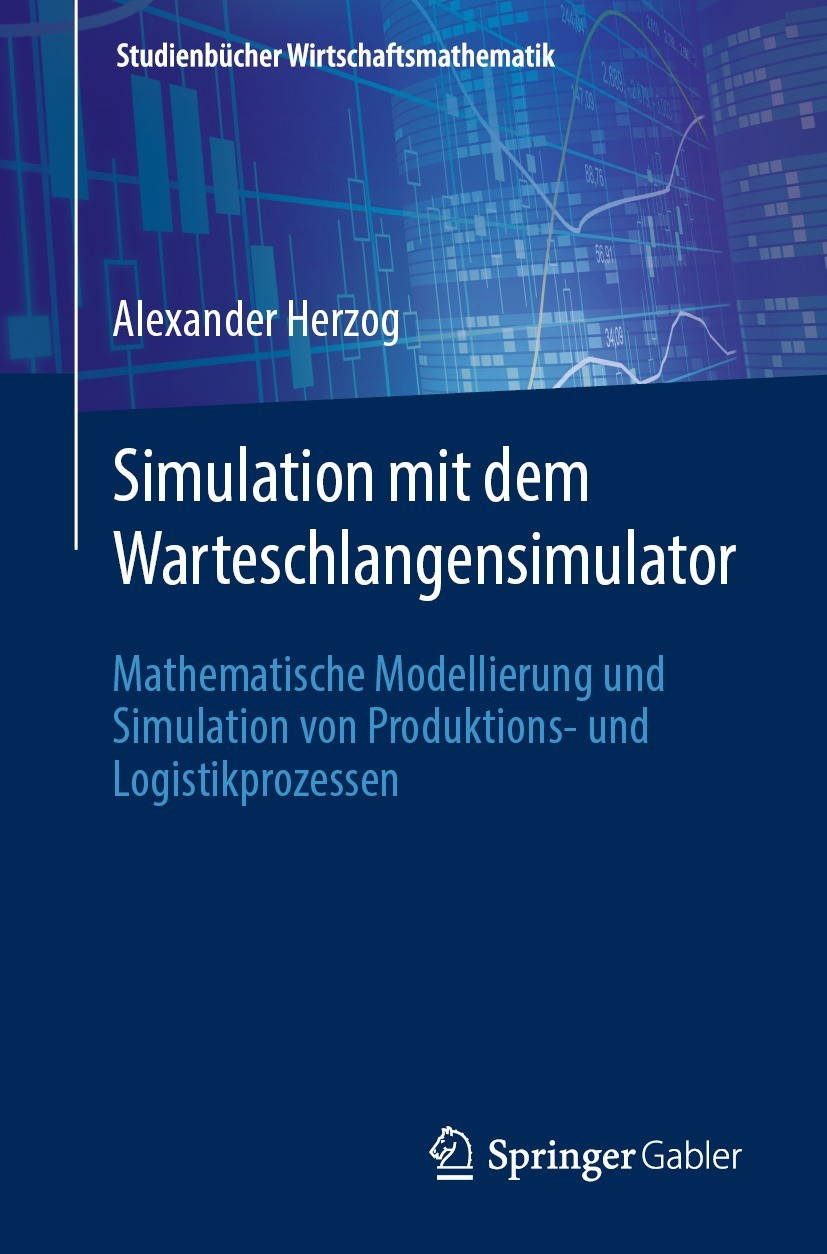
\includegraphics[width=6cm]{../BookCover.jpg}
\end{minipage}
\hfill
\begin{minipage}[b]{9.25cm}
Alexander Herzog:\\
\emph{Simulation mit dem Warteschlangensimulator},\\
Springer, 2021.
\vskip0.5em
ISBN: 978-3-658-34667-6
\vskip0.5em
\href{https://link.springer.com/book/10.1007/978-3-658-34668-3}{link.springer.com/book/10.1007/978-3-658-34668-3}
\end{minipage}

\end{document}